\documentclass{beamer}
%
% Choose how your presentation looks.
%
% For more themes, color themes and font themes, see:
% http://deic.uab.es/~iblanes/beamer_gallery/index_by_theme.html
%
\usetheme{Madrid}
%\mode<presentation>
%{
%  \usetheme{Boadilla}     % or try Boadilla, Darmstadt, Madrid, Warsaw, default, ...
%  \usecolortheme{default} % or try Boadilla, albatross, beaver, crane, default, ...
%  \usefonttheme{default}  % or try Boadilla, serif, structurebold, default, ...
%  \setbeamertemplate{navigation symbols}{}
%  \setbeamertemplate{caption}[numbered]
%} 

\usepackage{listings}

\usepackage{tikz}

\usepackage{movie15}
\usepackage{media9}

\usepackage{color}

 \usepackage{multirow}
 \usepackage[font=scriptsize]{caption}
 \usepackage{cite}
\usepackage{graphicx}
\usepackage{amsmath}
\usepackage{tikz}
\usepackage[font = small]{caption}

\usepackage[english]{babel}
\usepackage[utf8x]{inputenc}
\usepackage{color}

\title[IIT Hyderabad]{Local Server using Raspberry Pi}
%\subtitle{Lecture 1}
\author[ National Resource Centre] {Introduction IoT \& Robotics using Arduino }

\institute[]{\textbf{Dr. G.V.V.Sharma}}
\date{Dept. of Electrical Engineering}


\AtBeginSubsection[]
{
  \begin{frame}<beamer>{Outline}
    \tableofcontents[currentsection,currentsubsection]
  \end{frame}
}


\begin{document}

\begin{frame}
	\begin{center}
  \titlepage 
      \begin{figure}[h]
  
\includegraphics[width=2.8cm,height=2.3cm] {GIMG/iith.png}
      \end{figure}
  \end{center}
\end{frame}


\begin{frame}{Frame Title}
    
\end{frame}

\begin{frame}{Resource Persons}
\begin{center}
\begin{figure}
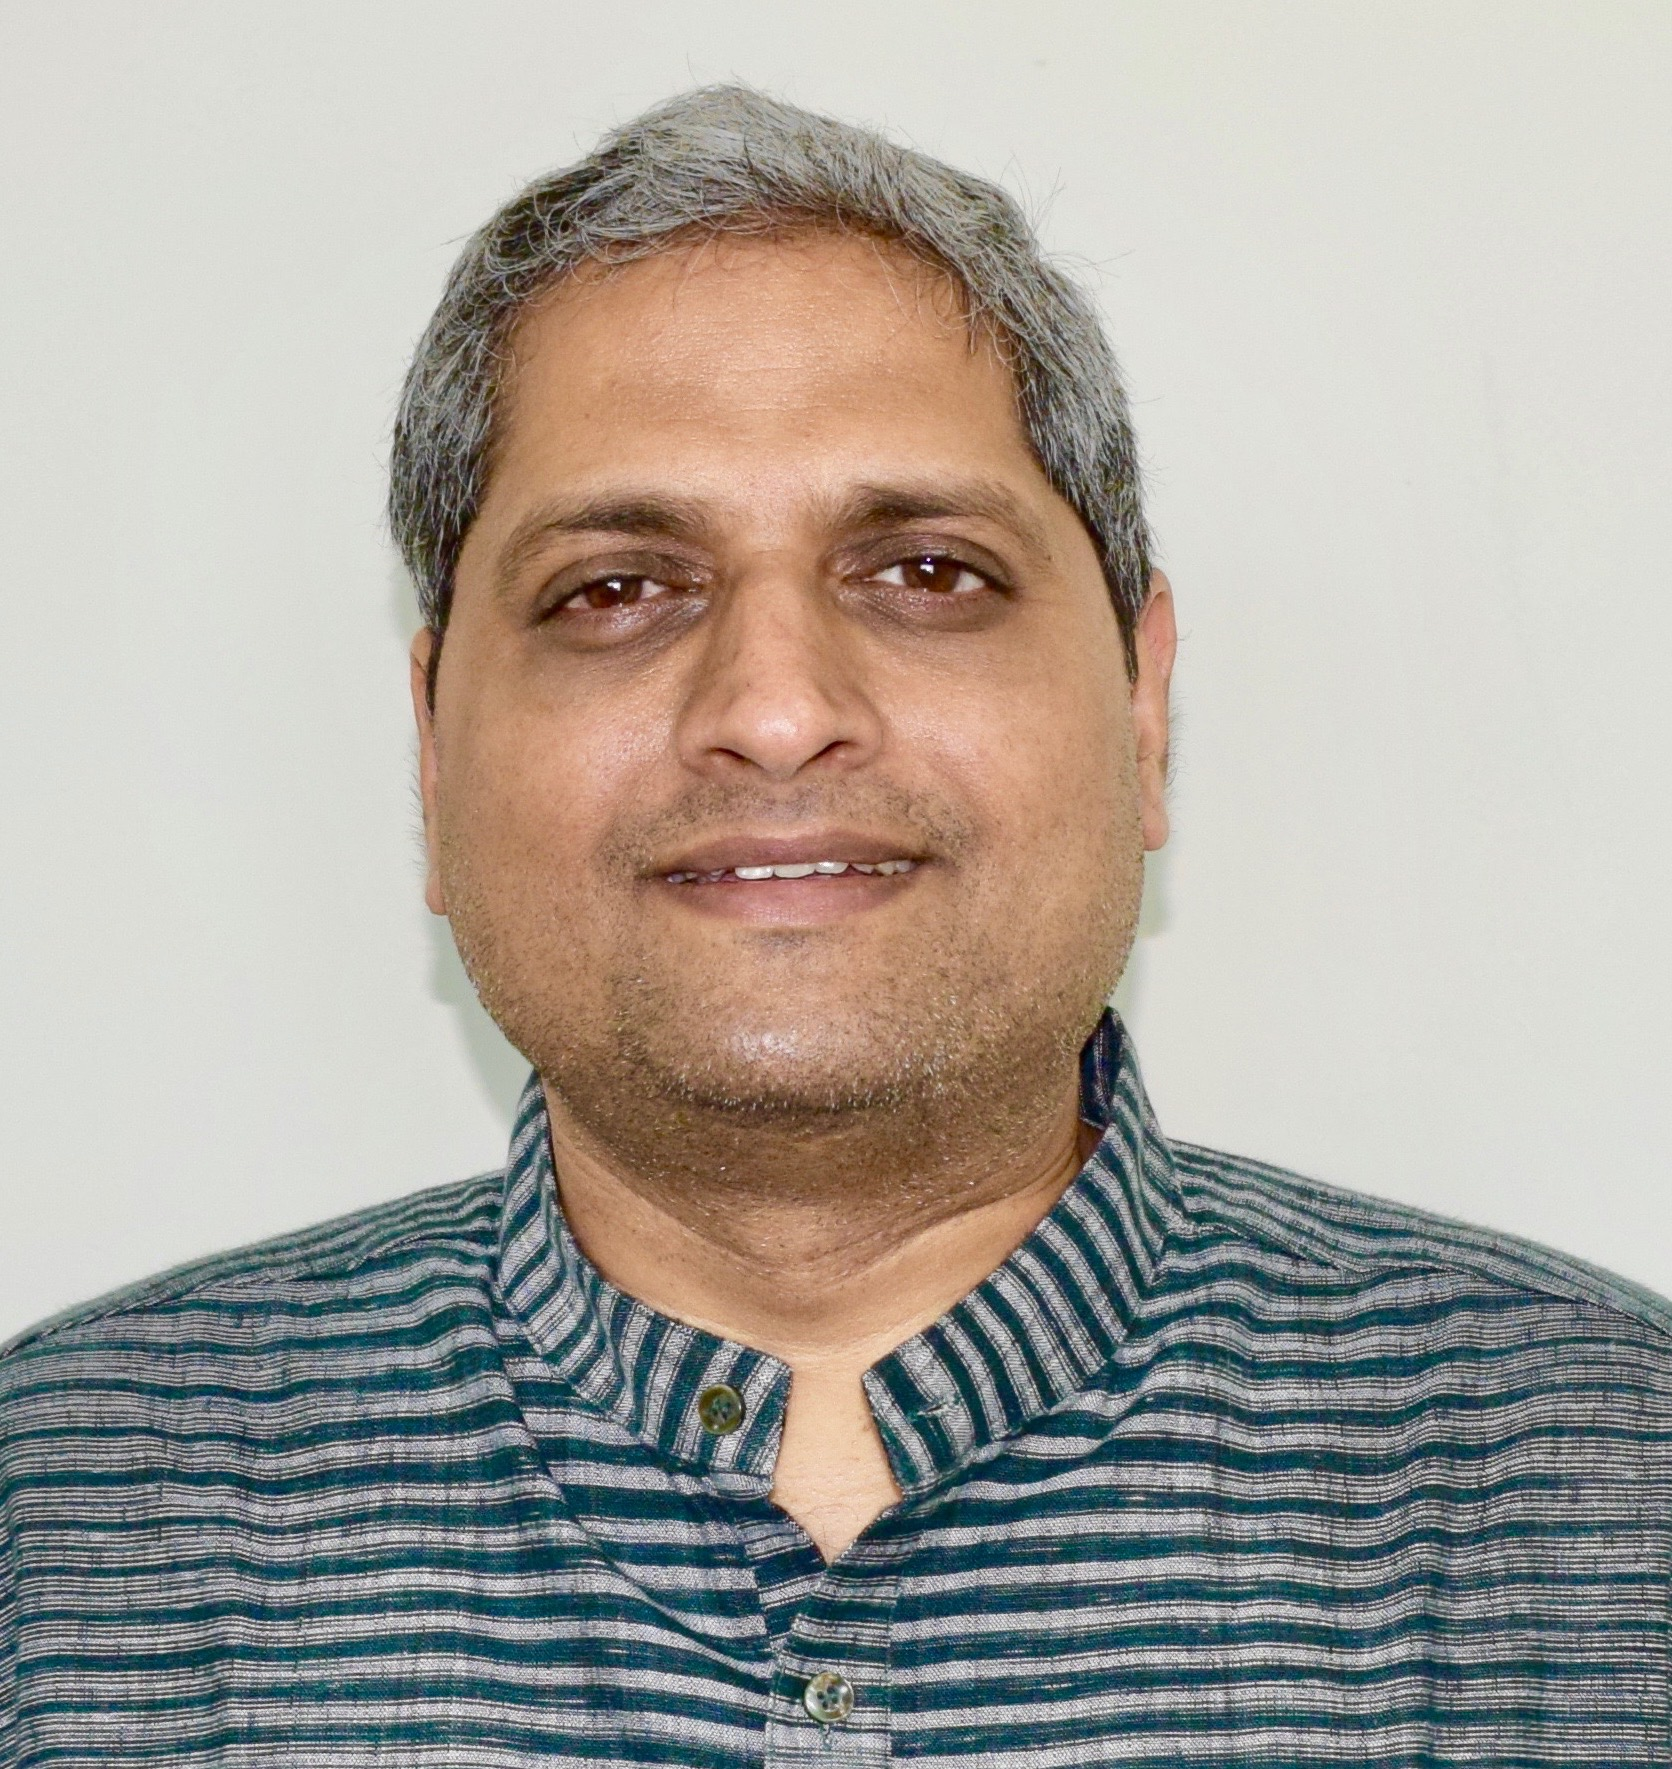
\includegraphics[scale=0.04]{GIMG/sharma.png}\\
Dr. G.V.V.Sharma\\
gadepall@iith.ac.in
\end{figure}
\vspace{0.75cm}
\begin{minipage}{0.47 \textwidth}
\begin{figure}
\centering
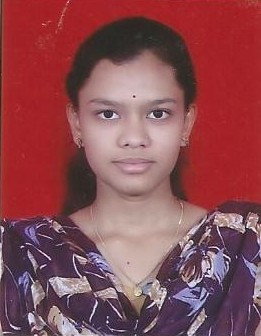
\includegraphics[width=2cm,height=2.1cm]{GIMG/Prakurti.jpg}\\
Prakruti M Bilagi\\
pmbilagi@gmail.com
\end{figure}
\end{minipage}
\begin{minipage}{0.5 \textwidth}
\begin{figure}
\centering
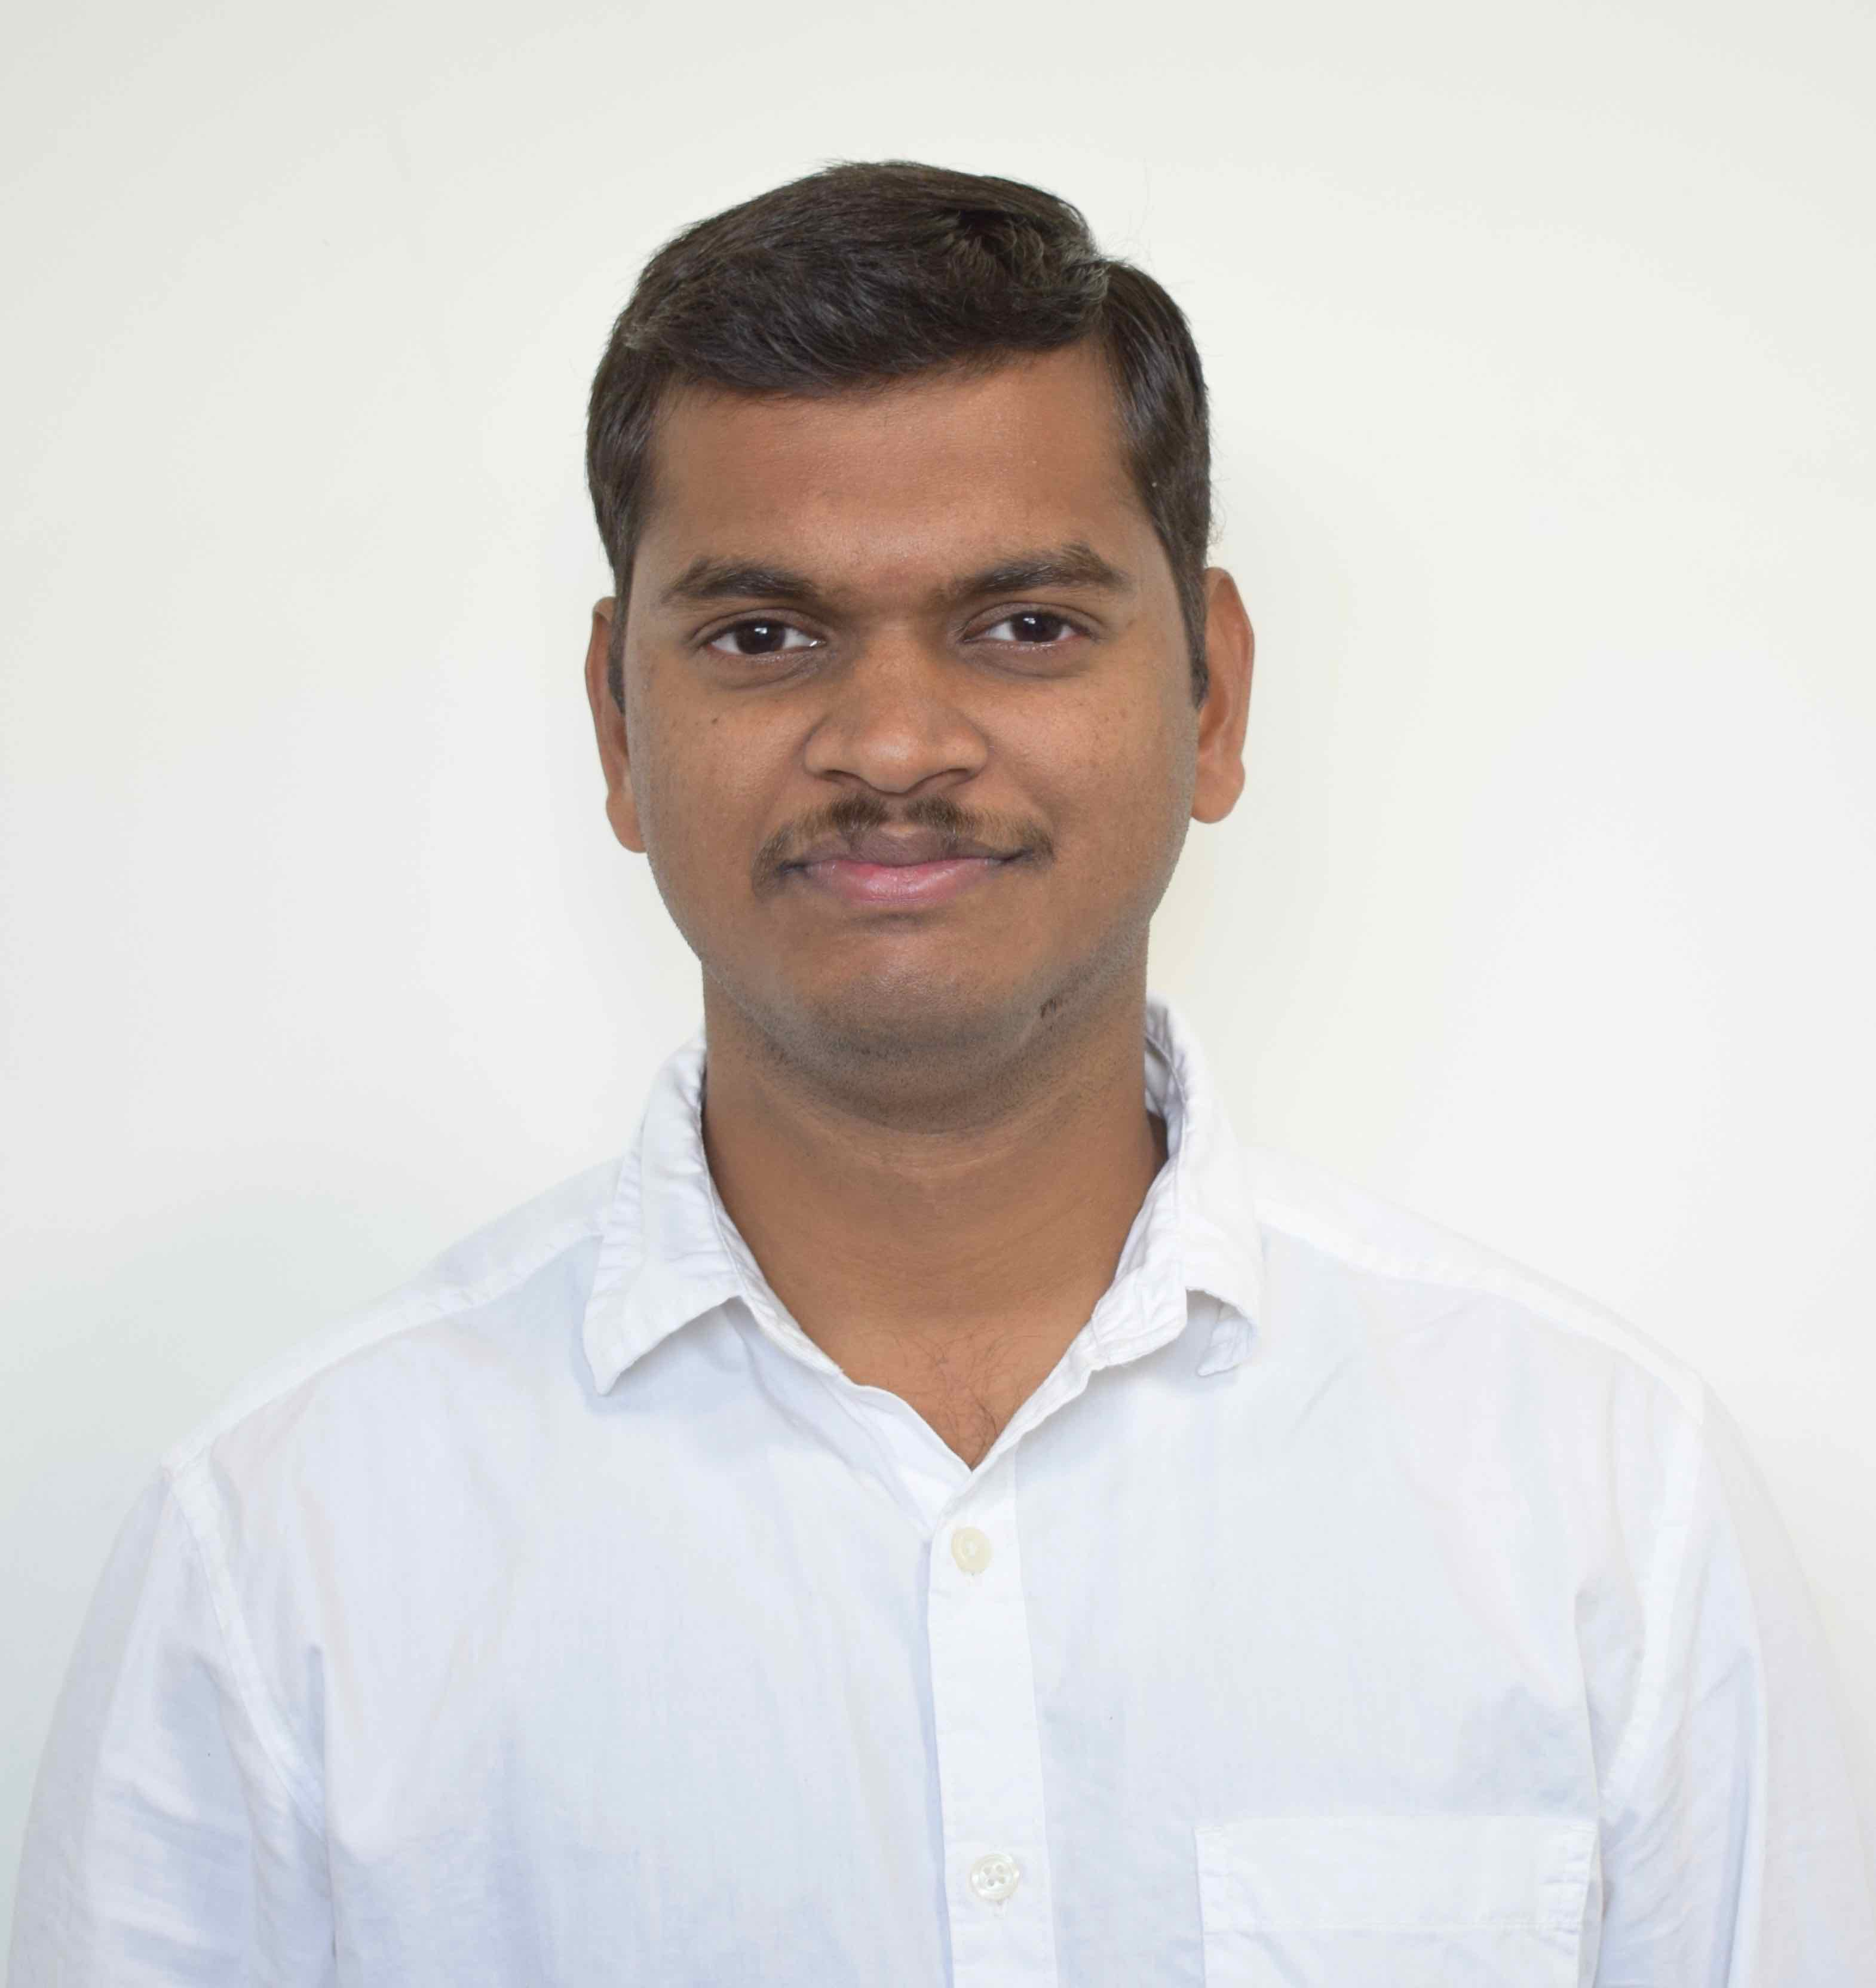
\includegraphics[width=2cm,height=2.1cm]{GIMG/Prasanna.jpg}\\
K. Prasanna Kumar\\
kprasannakumar@iith.ac.in
\end{figure}
\end{minipage}
\end{center}

\end{frame}



\begin{frame}{References}
\begin{thebibliography}{00}
\bibitem{b1} Electrical Engineering Repository, Teaching Learning Centre, IIT Hyderabad \\ \url{www.tlc.iith.ac.in/}
\bibitem{b2} Electrical Engineering National Resource Centre, IIT Hyderabad. \\ \url{www.nrc.iith.ac.in}

\end{thebibliography}
\end{frame}



\begin{frame}{Contact Details}
\onslide<1->
\vspace{1cm}
National Resource Centre,\\
Room No: 719, Academic Block A,\\
IIT Hyderabad,\\
Kandi, Sangareddy,\\
Telangana 502285
\onslide<2->
\vspace{0.5in}
\vfill
\begin{flushright}

\includegraphics[scale=0.7]{GIMG/thank.jpg}
\end{flushright}
\end{frame}

\end{document}
